\documentclass{article}
\usepackage[utf8]{inputenc}
\usepackage[T1]{fontenc}
\usepackage[french]{babel}
\usepackage[pdftex]{graphicx} % Figures
\usepackage{amsmath} % Accolades
\usepackage{amssymb} % pour N
\graphicspath{{images/}}
\usepackage{float} % Placement des images
\usepackage{geometry} %Marges
\geometry{
    hmargin=2.5cm,
    vmargin=2.5cm
}
\usepackage[onehalfspacing]{setspace} % Interlignes
\usepackage{calc}
\usepackage{caption} % Légende
\usepackage{subcaption} 
\usepackage{hyperref} % Hyperliens
\usepackage{fancyhdr} % En-têtes
\setlength{\headheight}{13pt}
\usepackage{listings} % Insertion de code

\newcommand{\HRule}{\rule{\linewidth}{0.5mm}}

\pagestyle{fancy}
\lhead{}
\rhead{}

\title{Génération procédurale}
\author{}
\date{}

\begin{document}


\begin{titlepage}
    \begin{center}
         %Logo
	    
\includegraphics[scale=0.5]{logo.jpg}

        \textsc{\LARGE\\[0.5cm]ENSEIRB-MATMECA}
        \\[0.5cm]
        \textsc{\LARGE Filière informatique}
        \\[2cm]

        % Titre
        \textbf{\LARGE \textsc{--Projet de programmation fonctionnelle--}}
        \\
        \textbf{\LARGE \textsc{--Semestre 6--}}
        	
        \HRule
        { \huge \textbf{Rapport de projet\\Génération Procédurale}}
        \\[0.25cm]
        \HRule
        \\[1.5cm]
    
        % Auteur
    	\textsc{\Large Théo GOMICHON\qquad}
    	\textsc{\Large Clément SACCOCCIO}\\[0.5cm]
    	\textsc{\Large Hugo LANGLAIS\qquad}
    	\textsc{\Large Faustin BOITEL}\\[0.5cm]
    	\textsc{\large Encadré par Mr. Morandat Floréal}
        \vfill
       
    	% Pied de page
        {\large \textsc{2020 — 2021}}
    \end{center}
\end{titlepage}

\section*{Introduction}
\paragraph{}
Ce rapport est le document explicatif du projet de programmation fonctionnelle de semestre 6 réalisé par l'équipe composée de Théo Gomichon, Clément Saccoccio, Hugo Langlais et Faustin Boitel. \\
Il porte sur le développement d'une bibliothèque de génération et traitement d'images en \textsf{JavaScript}.

\paragraph{}
Ce rapport est structuré dans une logique d'approfondissement progressif. Nous commencerons ainsi par expliquer brièvement les tenants et aboutissants du sujet.
Nous analyserons ensuite l'architecture de notre projet en réalisant une observation des différentes structures et interfaces mises en oeuvre.
Puis nous plongerons au coeur des détails techniques en présentant certains exemples d'implémentations.
Enfin nous conclurons par une prise de recul globale sur le projet, en présentant ses limites ainsi que les différents enseignements que nous avons pu tirer de ce travail. 

\newpage
\tableofcontents
\fancyhead[L]{\slshape \leftmark}
\newpage
TODO TRANSPARENCE REFERENTIELLE + fond vert

\section{Description du projet et son organisation}
\subsection{Génération procédurale}

La création d'objets manuellement peut être fastidieuse, c'est pourquoi la génération procédurale, est utilisée afin de créer des objets automatiquement. Cette méthode utilise des outils algorithmiques, il est donc très facile de produire des objets variés  et en grand nombre sans passer des heures sur un outil de création numérique. La génération procédurale est beaucoup utilisé pour la génération de textures afin de colorier des grandes zones 3D comme des forêts ou des routes.
Dans ce projet, nous allons développer une bibliothèque de génération procédurale d'image.

\subsection{Choix de l'équipe}

\paragraph{}
Nous avons décidés de réaliser notre projet en TypeScript, qui est pour nous un bon compromis entre la flexibilité du JavaScript et la lisibilité d'un langage typé.

\paragraph{}
Pour l'organisation, nous avions décidés de tenir un cahier de bord, dans lequel nous notions notre avancée à chaque fin de séance. L'objectif était d'avoir une trace de notre avancée afin de simplifier la rédaction du rapport. Après quelques semaines, le cahier de bord n'était plus mis à jour, ce qui avec le recul était une erreur.

\paragraph{}
Au niveau du développement, nous avons défini les éléments de base tous ensembles (image, couleur, générateur et filtre) afin que chaque membre ai bien compris le fondement de la bibliothèque. Nous nous sommes ensuite réparti les tâches entre l'implémentation des différents filtres et générateurs et le développement des interfaces Node.js et Web.

\section{Structure des éléments}

\paragraph{}
Le travail en équipe conjugué à l'utilisation d'un langage à typage fort tel que TypeScript nous a obligé à définir rapidement et de façon claire les différents éléments constituants le projet. Il a ainsi fallu caractériser les briques de base que sont les images et les couleurs qui les composent, puis les générateurs et les filtres composants notre bibliothèque, mais également les différentes interfaces nous permettant d' utiliser ces derniers correctement.

\subsection{Couleur}

Nous définissons une couleur suivant la notation RGBA. C'est un tableau de 4 valeurs entières allant de 0 à 255. Une couleur représentera un pixel de l'image.

\begin{equation*}
    Couleur = \left\{\begin{matrix}
            rouge \in \mathopen{[} 0~;~255 \mathclose{]}  \\
            vert \in \mathopen{[} 0~;~255 \mathclose{]}  \\
            bleu \in \mathopen{[} 0~;~255 \mathclose{]}  \\
            alpha \in \mathopen{[} 0~;~255 \mathclose{]}  \\
\end{matrix}\right.
\end{equation*}

Nous avons implémenté des fonctions de manipulation de couleur au fur et à mesure des besoins rencontrés lors du développement de la bibliothèque.

\subsection{Image}
\label{sec:image}

Il existe de nombreuses manière de représenter une image numériquement. Nous avions décidés de retenir deux implémentations : - représenter l'image par une matrice de pixels - représenter l'image par une fonction \\
Après réflexion, c'est finalement la dernière implémentation qui à été retenue. Elle semblait pour nous plus pratique à manipuler, bien que moins intuitive. Nous avons également besoins de stocker des informations sur l'image comme ses dimensions. Notre image est donc un objet ayant comme attribut sa largeur, sa hauteur et une fonction qui étant donné des coordonnées retourne une couleur.
\begin{equation*}
    Image = \left\{\begin{matrix}
            largeur \in \mathbb{N} \\
            hauteur \in \mathbb{N} \\ 
            f : \mathbb{N} \times \mathbb{N} \rightarrow Couleur
\end{matrix}\right.
\end{equation*}
 
\subsection{Générateur}

Un générateur est un constructeur d'image. Étant donné une largeur et une hauteur, il retourne une image. D'autres arguments propres au générateur peuvent être fournis comme par exemple des couleurs.

\begin{equation*}
    G\acute{e}n\acute{e}rateur = f : \mathbb{N} \times \mathbb{N} \times \dots \rightarrow Image
\end{equation*}

\subsection{Filtre}
\paragraph{}
On peut définir simplement un filtre comme une boîte noire prenant en entrée une image et renvoyant en sortie une autre image. Un filtre peut également prendre un nombre arbitraire d'arguments qui lui sont propres. Les arguments peuvent être d'autres images. De la sorte, il est possible de fusionner différentes images avec un filtre.

\begin{equation*}
    Filtre = f : Image \times \dots \rightarrow Image
\end{equation*}

\paragraph{}
Différents questionnement se sont posés sur la nature de ces transformations. Tout d'abord, étant dans une logique fonctionnelle, l'image renvoyée doit être une entité différente de l'image d'entrée afin de limiter les effets de bord. L'implémentation d'une image sous forme fonctionnelle vu en section \ref{sec:image} a permis de réaliser cela facilement. En effet, l'image étant caractérisée par sa taille et une fonction, il est trivial de copier la taille et de créer une nouvelle fonction par composition.

\paragraph{}
À l'instar des générateurs, dans notre implémentation fonctionnelle les filtres renvoient également une nouvelle entité représentant une image. Ainsi ce sont également des constructeurs d'image. Cependant un générateur construit son image à partir de paramètres données par l'utilisateur tandis qu'un filtre se base sur une image déjà existante.
On peut donc schématiser le processus fonctionnelle de génération d'image avec un générateur en début de file auquel il est possible de chaîner une infinité de filtres.

\begin{equation*}
    G\acute{e}n\acute{e}rateur \rightarrow Filtre \rightarrow \dots \rightarrow Filtre \rightarrow Image
\end{equation*}

\subsection{Interfaces Node.js et Web}
Nous avons implémenté les interfaces Node.js et Web. Même si Les deux interfaces sont très différentes, elles ont tout de même des bases communes, comme par exemple la définition d'une image. Nous avons voulu limiter au maximum la duplication de code. Une image peut être décrite par un fichier JSON, qui contient la suite de filtres et générateurs à appliquer afin d'avoir l'image finale.

Afin de simplifier le développement, nous avons mit en place des script de ...

L'interface node fonctionne à partir de la ligne de commande. 
Nous pouvons passer en argument le fichier JSON qui décrit l'image à créer. Le résultat est ensuite sauvegardé en PNG dans le dossier public.

La version web sert principalement aux tests, afin d'avoir un visuel

--> diff + ptn communs centralisation 
--> création à partir d'un json
--> mise en place des règles npm, parcel


\section{Analyse technique}

Plusieurs exemples de filtres et générateurs sont donnés dans le sujet. Dans cette partie, nous présentons nos implémentations, et comment elles s'adaptent, ou non, à nos structures.

\subsection{Générateurs}

Les générateurs permettent de créer une image à partir certains de paramètres. Nous présentons ici 4 générateurs d'images, le pavage du plan, les diagrammes de Vorinoi. 

\subsubsection{Pavages réguliers, semi-réguliers et pentagonaux du plan}
Dans un premier temps, le sujet nous a amené à nous questionner sur comment nous pourrions réaliser différents pavages du plan, tels que les pavages réguliers, semi-réguliers où encore pentagonaux. Pour mener à bien ces réalisations, deux approches différentes ont été abordées, l'une se prêtant parfaitement à nôtre conception d'image en tant que fonction, l'autre un peu moins.
\begin{enumerate}
    \item \textbf{Première méthode} 
    
\hspace*{0.5cm}La première approche s'appuie sur le caractère répétitif, les symétries que présentent certains pavages ainsi que la possibilité de pouvoir caractériser avec des équations les droites du pavage. Pour mieux comprendre comment ce procédé fonctionne, chaque étape sera décrite et illustrée avec un exemple, ici la réalisation du pavage triangulaire, que l'on peut observer sur la Figure~\ref{fig:pavage_triangle}.

\hspace*{0.5cm}\hspace*{0.5cm}La première étape de cette approche est alors de définir une portion rectangulaire caractéristique du pavage, à savoir qui se répète partout dans le pavage, et de placer un repère. Cette zone est délimité par des traits pointillés rouges sur la Figure~\ref{fig:pavage_triangle}. Ainsi, si l'on connaît la couleur associé à chaque pixel de cette zone alors on connaît la couleur de chaque pixel du plan, en utilisant l'opération \textbf{modulo} sur les réels. Pour l'exemple du triangle, en prenant comme unité la longueur d'un coté d'un triangle, la hauteur de ce triangle est alors égale à $\sin \left(\frac{\pi}{3}\right)$,et on à alors l'affirmation suivante : 
\begin{equation*}
    \forall \: x, y \in\ ]-\infty, \infty[,\ Couleur(x,\ y)\ =\ Couleur \left(x \mod 1,\ y \mod \left(2.\sin\frac{\pi}{3} \right)\right)
\end{equation*}

\hspace*{0.5cm}Ensuite, lorsque l'on a déterminé une telle zone, on peut encore chercher des symétries à l'intérieur afin de simplifier encore davantage la procédure. Ici, deux plan de symétrie, dessinés en vert sur la Figure~\ref{fig:pavage_triangle}, sont présents : le plan d'équation $x = \frac{1}{2}$ et le plan d'équation $y = \sin\frac{\pi}{3}$. On peut alors ramener $x$ et $y$ dans cette zone réduite, en pensant à prendre en compte le fait que les couleurs soient inversées pour la symétrie par rapport au plan $y = \sin\frac{\pi}{3}$. 

\hspace*{0.5cm}Finalement, n'ayant plus qu'à déterminer la valeur de $Couleur(x,\ y)$ sur une zone minimale, on utilise les équations des droites traversant cette zone pour obtenir des conditions sur $x$ et $y$. Dans notre exemple du pavage triangulaire, une droite coupe cette zone, et en utilisant les propriétés géométriques, l'équation de cette droite est $y\ = \ 2.\sin \left((\frac{\pi}{3} \right).x$, en bleu sur l'illustration.
En considérant ces deux derniers aspects, les couleurs des pixel délimités par les droites vertes sont alors :

\begin{equation*}
    \forall x \in \left[0, \frac{1}{2}\right], \forall y \in [0, \sin\left(\frac{\pi}{3} \right)], \left\{\begin{matrix}
            Couleur(x, y) = couleur1\ si\ y > 2.\sin \left(\frac{\pi}{3} \right).x  \\
            Couleur(x, y) = couleur2\ si\ y < 2.\sin \left(\frac{\pi}{3} \right).x  \\
\end{matrix}\right.
\end{equation*}

\begin{figure}
    \centering
    \includegraphics[width=13cm]{Caractérisation du pavage triangulaire.png}
    \caption{Caractérisation du pavage triangulaire}
    \label{fig:pavage_triangle}
\end{figure}


\hspace*{0.5cm}Cette méthode convient parfaitement à notre implémentation de l'image, car on peut accéder à la couleur de n'importe quel pixel du plan en temps constant. Elle a notamment permis de réalisé les pavages réguliers  carré, triangulaire et hexagonal, mais aussi des pavages semi-réguliers tels que les pavage carré adouci ou encore le pavage grand rhombitrihexagonal (Voir annexe) . Cependant, cette méthode possède des limites, typiquement lorsque le pavage se présente pas de symétrie ou bien lorsque les motifs sont trop complexes et deviennent difficilement modélisables par des équations. 

\item \textbf{Seconde méthode}

\hspace*{0.5cm}Cette approche a été développée essentiellement pour répondre à la problématique de la génération du pavage pentagonal. Les pavages pentagonaux consistent à recouvrir le plan cartésien par un unique  pentagone que l'on duplique. Les pavages pentagonaux sont classé en différents types, selon les propriété du pentagone et donc des agencements possible qui en découlent. A titre d'exemple, le pentagone de type 1, dont une représentation est en Figure~\ref{fig:pent1}, possède la propriété suivante : ses coté a et c sont parallèles. A partir de ce derniers, on pourra générer une infinité de pavage que l'on dira de type 1, en faisant simplement varier les longueurs a, b, c et d ainsi que les angles A et C, et aussi en choisissant la manière dont on disposera les tuiles. Un exemple est donné en Figure~\ref{fig:pavage_pent1}, avec comme paramètres :
\begin{equation*}
    \left\{\begin{matrix}
                b = 1,1.a \\ 
                c = 0,7.a \\
                d = 0,7.a \\
                \hat{A} = 100 \deg \\
                \hat{B} = 130 \deg \\
\end{matrix}\right.
\end{equation*}

et en disposant les pentagone de la façon suivante : on prend un second pentagone qui est une rotation à 180 $\deg$ du premier, on accole leurs coté b, puis on calque le motif obtenu sur tout le plan.

\begin{figure}
    \centering
    \begin{subfigure}{0.44\textwidth}
        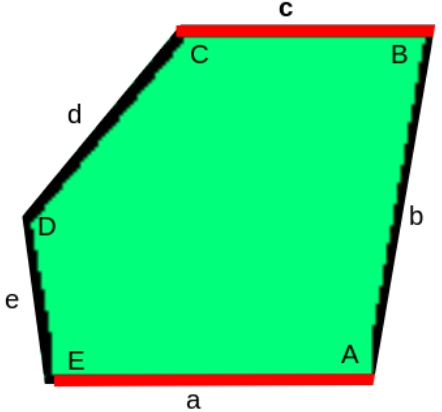
\includegraphics[width=\textwidth]{pentType1.png}
        \caption{Pentagone de type 1}
        \label{fig:pent1}
    \end{subfigure}
    \begin{subfigure}{0.44\textwidth}
        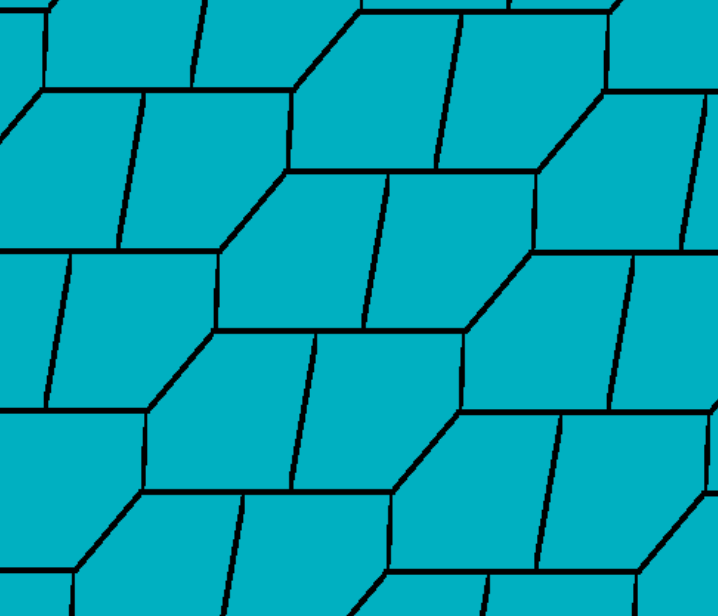
\includegraphics[width=\textwidth]{pavagePentType1.png}
        \caption{Un pavage pentagonal de type 1}
        \label{fig:pavage_pent1}
    \end{subfigure}
    \caption{Caractérisation du pavage pentagonal de type 1}
    \label{fig:carpent1}
\end{figure}



\hspace*{0.5cm}Ainsi, voyons pour commencer comment générer un tel pentagone. L'idée est la suivante, on part d'un point initial quelconque, puis on construit progressivement le premier pentagone. De cette façon, on peut connaître les coordonnées de chaque sommet, car pour aller d'un point A à un point B distants de l, si la droite (A, B) pour un angle $\theta$ avec l'axe des abscisses, en utilisant la trigonométrie, les coordonnées de B sont les suivantes : 
\begin{equation*}
        \left\{\begin{matrix}
        x_b = x_a + l.\cos{\theta} \\
        y_b = y_a + l.\sin{\theta} \\
\end{matrix}\right.
\end{equation*}
\hspace*{0.5cm}Au niveau de l'implémentation, partant d'un tableau dont le premier élément désigne les coordonnées du premier points, et les éléments suivant les couples (angle, distance) pour aller de points en points, l'opérateur \texttt{map} convient parfaitement pour transformer ce tableau en un tableau de coordonnées. 


\hspace*{0.5cm}Connaissant maintenant les coordonnées de chaque sommet, on peut facilement connaître l'équation d'une droite reliant deux d'entre eux. En parcourant ces derniers deux à deux dans l'ordre, on peut alors déterminer si oui où non un point quelconque de coordonnées (x, y) est à un $\epsilon$ près de la droite. On vient alors de construire le premier pentagone.

\hspace*{0.5cm}Pour le "retourner", il suffit d'appliquer le même algorithme avec des distances négatives. Désormais, après avoir déterminer le point d'origine de chaque pentagone dans le plan (que l'on ferra une fois de plus par construction géométrique, mais que l'on ne détaillera pas ici pour éviter les redondances), on construit les pentagones, et on obtient un pavage pentagonal du plan.

\hspace*{0.5cm} Cependant, notre implémentation présente un problème : du fait que pour chaque pixel, nous devons vérifier si oui ou non il se trouve sur l'une des arêtes de l'un des pentagones, cela implique la construction virtuelle de chaque pentagone pour tester chaque pixel. Cela le rend assez long à l'exécution pour des tailles d'images assez grandes. Ainsi, malgré un pavage obtenu très juste, implémentée de cette façon, cette méthode ne s'adapte pas parfaitement à notre représentation de l'image. Avec un peu plus de temps nous aurions peut-être pu la mettre en place différemment, notamment en ne construisant qu'une seule fois les polygones, puis en les stockant par exemple en utilisant la mémoïzation (Nous aurons l'occasion de revenir sur cette methode en 3.1.4).

\end{enumerate}

\subsubsection{Bruit fractal}

\subsubsection{Diagrammes de Voronoi}

Des points sont placés aléatoirement sur l'image, appelés germes. Chaque germe est associé à une couleur. La couleur de chaque point de l'image est celle du germe le plus proche. Nous pouvons obtenir des images comme illustrés figure \ref{fig:voronoi_examples}.

\begin{figure}[h]
    \centering
    \begin{subfigure}{0.3\textwidth}
        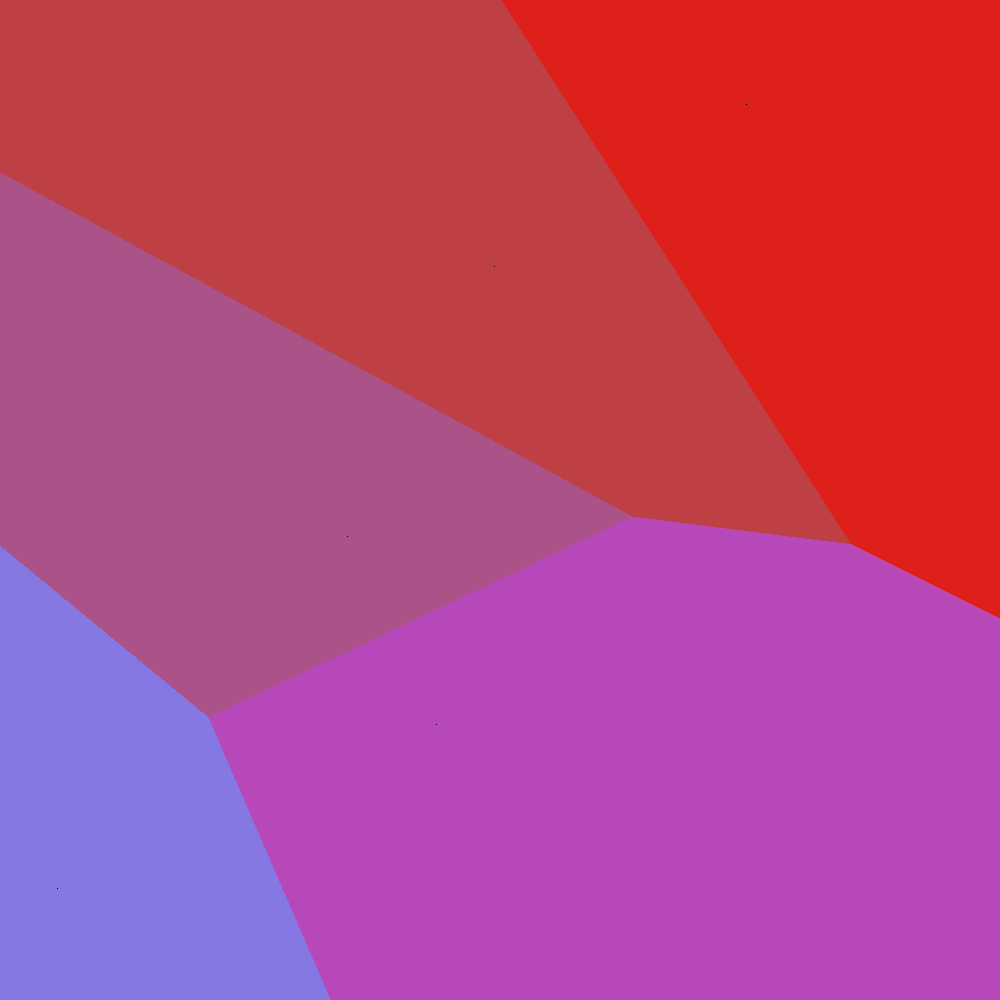
\includegraphics[width=\textwidth]{voronoi_5.png}
        \caption{Voronoi 5 points}
        \label{fig:voronoi_5}
    \end{subfigure}
    \begin{subfigure}{0.3\textwidth}
        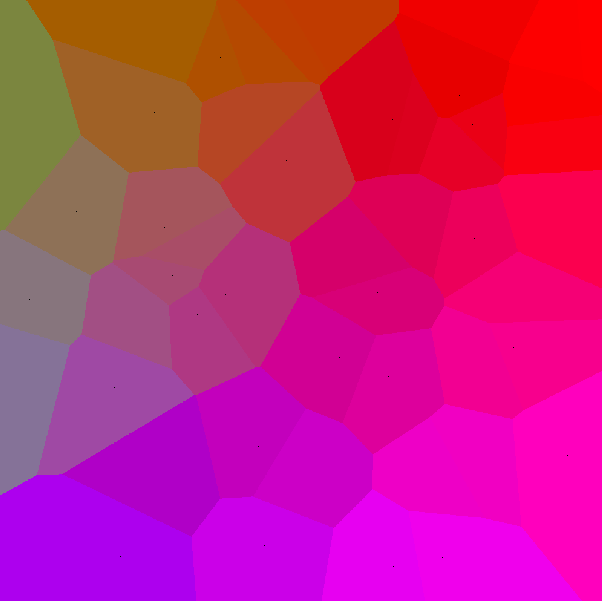
\includegraphics[width=\textwidth]{voronoi_50.png}
        \caption{Voronoi 50 points}
        \label{fig:voronoi_50}
    \end{subfigure}
     \begin{subfigure}{0.3\textwidth}
        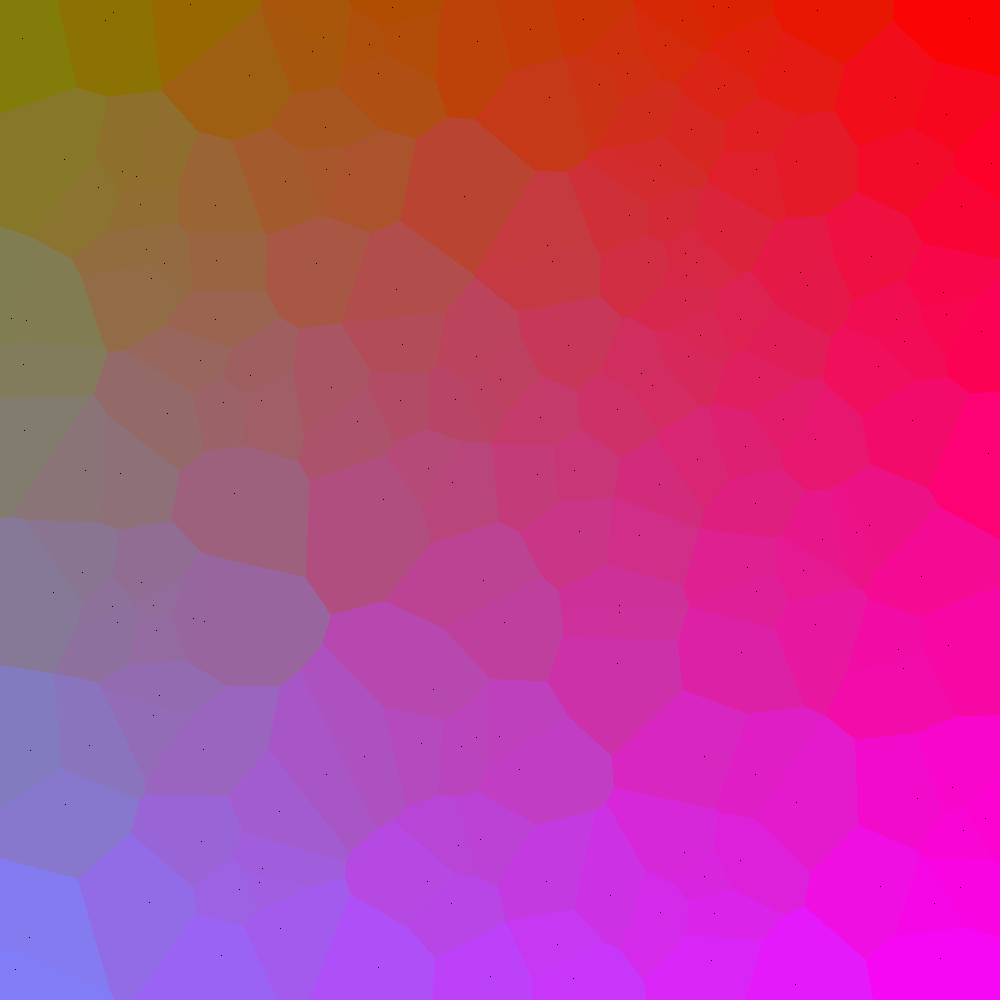
\includegraphics[width=\textwidth]{voronoi_200.png}
        \caption{Voronoi 200 points}
        \label{fig:voronoi_200}
    \end{subfigure}
    \caption{Diagrammes de voronoi pour 5, 50 et 200 points}
    \label{fig:voronoi_examples}
\end{figure}

Afin d'avoir un meilleur visuel, les couleurs des germes dépendent de leur position, ainsi, deux germes proches auront des couleurs proches. Ceci permet de limiter les cassures de couleurs. Plus le nombre de points augmente, plus l'image générée ressemble à un dégradé. Ce type de génération peut être utilisé afin d'habiller une route de pavés.

La position et la couleur de tous les germes sont enregistré dans une liste. Quand la couleur d'un point est demandée, on calcul la distance par rapport à tous les germes, puis on en détermine le germe le plus proche et on retourne sa couleur. Pour une image de taille n $\times$ m   
\subsubsection{Feu de forêt}
Un automate cellulaire est un ensemble de cellules dans un certain état, qui évolue au cours du temps en fonctions de l'état précédent de l'automate. Le modèle du feu de forêt est un automate cellulaire dont trois états sont possibles pour une cellule : un arbre, un emplacement vide ou un feu. Ses règles pour passer d'un état à l'autre sont les suivantes : 
\begin{itemize}
    \item Un emplacement vide se transforme en arbre avec une probabilité p;
    \item Un arbre s'enflamme s'il est en contact avec au moins un autre arbre enflammé;
    \item Un arbre s'enflamme seul avec une probabilité f;
\end{itemize}

Pour transformer ceci en image, nous donnerons bien-sûr une couleur pour chaque état.

\subsection{Filtres}

Les filtres se basent sur une image déjà existante. Ainsi les différentes techniques de filtrage ont mis à l'épreuve l'implémentation de nos éléments.

\subsubsection{Convolution}
La convolution est le processus consistant à ajouter chaque pixel de l'image à ses voisins, pondéré par les éléments d'une matrice appelée noyau.
Le problème qui se pose alors est qu'après
Or comme notre implémentation de filtre construit sa propre image le problème ne se pose pas.

\subsubsection{Composition}
si 2 images on pas la même taille ? 

\subsubsection{Redimensions}


\subsection{Comment combiner efficacement tout ça ?}
-> accent sur la combinaison fonctionnelle

annexe : exemples d'images

\subsection{Difficultés / limites du projet}

\section*{Conclusion}
Goodbye world


\end{document}
